\documentclass[11pt,reqno]{amsbook}

\usepackage{../HBSuerDemir}
\begin{document}

    \setcounter{chapter}{1}
    \chapter{\large INTEGRATION \\ (FUNCTIONS OF SEVERAL VARIABLES)}
    
    \hPage{b2p2/362}

    \setcounter{section}{4}
    \section{I. LINE INTEGRALS (CURVILINEAR INTEGRALS)}
    
    \qquad A. DEFINITIONS \\
    
    \qquad Let
    
    \begin{align*}
        F(x, y, z) = P(x, y, z)i + Q(x, y, z)j + R(x, y, z)k   
    \end{align*}
    
    \begin{flushleft}
        be a vector function on a domain D$\varepsilon R^3$.By $F$, to each point $(x, y, z)$ of D, there is assigned a single vector $Pi+Qj+Rk$.The set of all these vectors are said to form a \textit{vector field F}.
    \end{flushleft}
    
    Let $\Gamma$ be a curve lying entirely in D. Then the (indefinite) integral.
    
    \begin{align}
        \int_{\Gamma} Pdx + Qdy + Rdz\tag{1}
    \end{align}
    
    \begin{flushleft}
        is called a \textit{line Integral (curvilinear integral)} along $\Gamma$ (the point $(x, y, z)$ varies on $\Gamma$), where $\Gamma$ is considered as \textit{path} of the point $(x, y, z)$.
    \end{flushleft}
    
    \begin{minipage}{0.6\textwidth}
    \quad If the integral is taken from a point A to a point B on $\Gamma$, (1) becomes a definite integral denoted by. \\
    
    \centering$\int_{A\Gamma}^{B} Pdx + Qdy + Rdz$
	\end{minipage}
	\hfill
	\begin{minipage}{0.4\textwidth}
	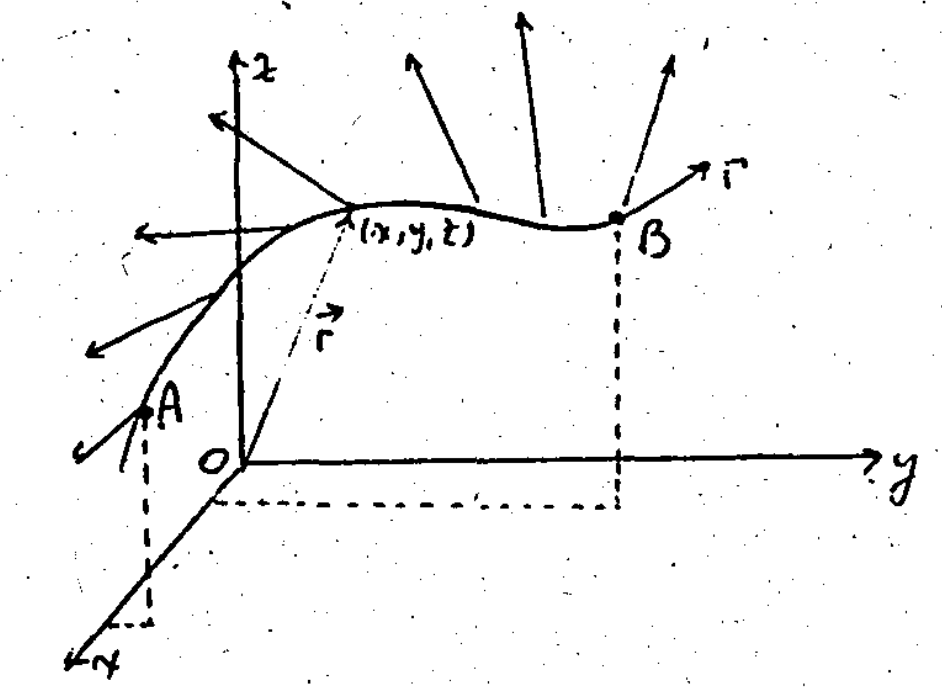
\includegraphics[width=\textwidth]{images/b2p2-362-fig01.png}
	\end{minipage}
	
	\begin{center}
        $\oint Pdx + Qdy + Rdz$
    \end{center}
	
	\begin{flushleft}
	    indicates that $\Gamma$ is a closed curve and the integral is taken for a complete revolution on $\Gamma$ in one of two senses.
	\end{flushleft}
	
	The line integral (1) can be written as 

\end{document}